\documentclass{article}
\usepackage{relsize}

\usepackage[utf8]{inputenc}
\usepackage{fancyhdr}
\usepackage{listings}
\usepackage{graphicx}
 
\pagestyle{fancy}
\fancyhf{}
\lhead{Exercise Sheet 3}
\rhead{Tim Schmiedl}
\rfoot{Page \thepage}

\begin{document}
\title{Data Analysis and Query Languages \\
 Exercise Sheet 3}
\date{\today}
\author{Tim Schmiedl} 
\maketitle

%%%%%%%%%%%%%%%%%%%%%%%%%%%%%%%%%%%%%%%%%%%%%%%%%%%%%%%%%%%%%
%%%%%%%%%%%%%%%%%%%%%%%%%%%%%%%%%%%%%%%%%%%%%%%%%%%%%%%%%%%%%
\section*{Exercise 1}
\lstinputlisting{ex3/ex1.txt} 


\vspace{2cm}
%%%%%%%%%%%%%%%%%%%%%%%%%%%%%%%%%%%%%%%%%%%%%%%%%%%%%%%%%%%%%
%%%%%%%%%%%%%%%%%%%%%%%%%%%%%%%%%%%%%%%%%%%%%%%%%%%%%%%%%%%%%
\section*{Exercise 2}
\subsection*{a) RDF Graph}
\begin{figure}[h!]
    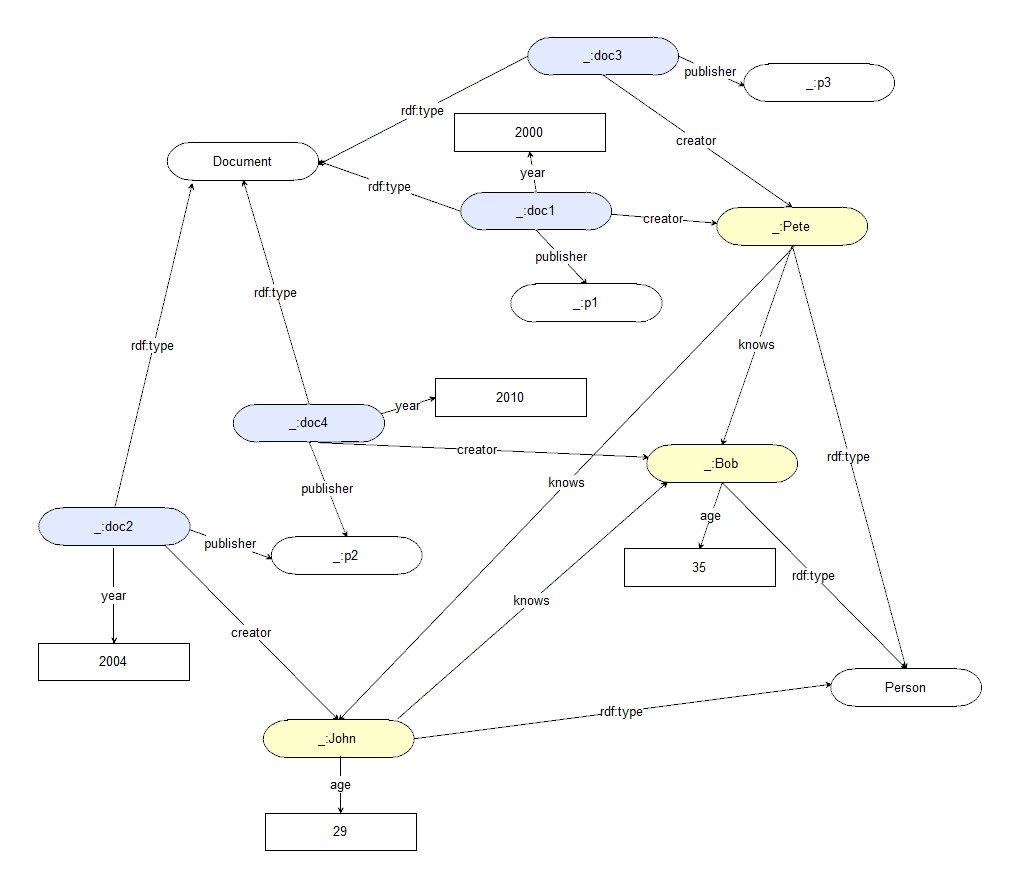
\includegraphics[width=1.2\textwidth]{img/rdf-graph.png}
\end{figure}

\subsection*{b) SPARQL}
\vspace{0.3cm}
(a) All Documents that are published after the year 2000.\\
\textbf{Result}: \{( :doc2, 2004), ( :doc4, 2010)\}\\
\vspace{0.3cm}

(b) All persons, if the person has an age given, show it too.\\
\textbf{Result}: \{( :John, 29), ( :Bob, 35), ( :Pete, )\}\\
\vspace{0.3cm}

(c) Persons for which an age is given or are the creator of something.\\
\textbf{Result}: \{( :John, 29) , ( :Bob, 35) , ( :Pete, :doc1) , ( :Pete,
:doc3) , ( :Bob, :doc4), ( :John, :doc2)\}
\vspace{0.3cm}

\vspace{2cm}
%%%%%%%%%%%%%%%%%%%%%%%%%%%%%%%%%%%%%%%%%%%%%%%%%%%%%%%%%%%%%
%%%%%%%%%%%%%%%%%%%%%%%%%%%%%%%%%%%%%%%%%%%%%%%%%%%%%%%%%%%%%
\section*{Exercise 3}
\subsection*{a)}
\subsubsection*{Query}
\begin{lstlisting}
SELECT * WHERE {
	?p rdf:type myns:Person .
	?d1 rdf:type myns:Document .
	?d2 rdf:type myns:Document .
	?d1 myns:creator ?p.
	?d2 myns:creator ?p.
	
	Filter (?d1 != ?d2)
}
\end{lstlisting}
\subsubsection*{Result}
\begin{lstlisting}
:Pete	:doc1	:doc3
:Pete	:doc3	:doc1
\end{lstlisting}




\subsection*{b)}
\subsubsection*{Query}
\begin{lstlisting}
select distinct ?p1 ?d ?a where {
{
	?p1 rdf:type myns:Person .
	?p2 rdf:type myns:Person .
	?p1 myns:knows ?p2 .
	?d myns:creator ?p1
	OPTIONAL {?p1 myns:age ?a}
}
UNION
{
	?p1 rdf:type myns:Person .
	?p1 myns:age ?age .
	?d myns:creator ?p1
	OPTIONAL {?p1 myns:age ?a}
	Filter (?age > 30)
}
}
\end{lstlisting}
\subsubsection*{Result}
\begin{lstlisting}
:Pete	:doc1	
:Pete	:doc3	
:John	:doc2	29
:Bob	:doc4	35
\end{lstlisting}


\subsection*{c)}
\subsubsection*{Query}
\begin{lstlisting}
SELECT ?pub ?age
WHERE
{
	?doc myns:publisher ?pub.
	?doc myns:creator ?creator.

	OPTIONAL{ ?doc myns:year ?date.}
	OPTIONAL{ ?creator myns:age ?age .}
	
	FILTER(!bound(?date))
}
\end{lstlisting}
\subsubsection*{Result}
\begin{lstlisting}
:p3
\end{lstlisting}


\vspace{2cm}
%%%%%%%%%%%%%%%%%%%%%%%%%%%%%%%%%%%%%%%%%%%%%%%%%%%%%%%%%%%%%
%%%%%%%%%%%%%%%%%%%%%%%%%%%%%%%%%%%%%%%%%%%%%%%%%%%%%%%%%%%%%
\section*{Exercise 4}
\small
\begin{tabular}{ l | l | l | l |}
& Sim & $URI_1$ & $URI_2$  \\
  \hline          
Top 1 & 74,62 & http://dbpedia.org/resouce/Sam\_Cooke &
http://dbpedia.org/resouce/Otis\_Redding \\
Top 2 & 72,28 & http://dbpedia.org/resouce/Ray\_Charles &
http://dbpedia.org/resouce/Little\_Richard \\
Top 3 & 70,74 & http://dbpedia.org/resouce/James\_Brown &
http://dbpedia.org/resouce/Little\_Richard \\
Top 4 & 63,81 & http://dbpedia.org/resouce/Sam\_Cooke &
http://dbpedia.org/resouce/Little\_Richard \\
Top 5 & 55,68 & http://dbpedia.org/resouce/Aretha\_Franklin &
http://dbpedia.org/resouce/Otis\_Redding \\
Top 6 & 48,33 & http://dbpedia.org/resouce/Al\_Green &
http://dbpedia.org/resouce/Otis\_Redding \\
Top 7 & 39,17 & http://dbpedia.org/resouce/Bob\_Dylan &
http://dbpedia.org/resouce/Otis\_Redding \\
Top 8 & 36,92 & http://dbpedia.org/resouce/Stevie\_Wonder &
http://dbpedia.org/resouce/Al\_Green \\
Top 9 & 35,85 & http://dbpedia.org/resouce/Al\_Green &
http://dbpedia.org/resouce/Smokey\_Robinson \\
Top 10 & 35,10 & http://dbpedia.org/resouce/Ray\_Charles &
http://dbpedia.org/resouce/Sam\_Cooke \\
  \hline  
\end{tabular}


\end{document}
